\begin{figure}[!ht]
	\centering
	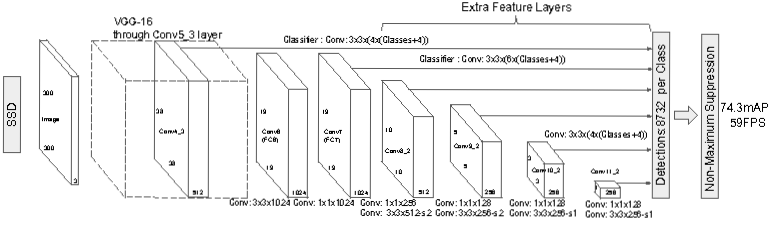
\includegraphics[width=0.8\textwidth]{chapter2/images/vgg.jpg}
		\caption[โครงสร้างทั่วไปของโมเดลปัญญาประดิษฐ์ SSD]{โครงสร้างทั่วไปของโมเดลปัญญาประดิษฐ์ SSD\textsuperscript{\cite{ssd_yolo_pic}}}
    	\label{fig:ssd}
\end{figure}

SSD\textsuperscript{\cite{liu2016ssd}} เป็นโมเดลปัญญาประดิษฐ์ที่ใช้โครงข่ายประสาทเทียมตัวเดียวสำหรับการตรวจจับวัตถุ ซึ่งภายในโครงข่ายจะประกอบไปด้วยการทำงานหลัก 3 อย่าง คือ
\begin{enumerate}
	\setlength\itemsep{-0.25em}
	\item การสกัดคุณลักษณะ\\
	นำภาพผ่าน VGG-16\textsuperscript{\cite{vgg}} (โมเดล CNN ชนิดหนึ่ง) เพื่อการสกัดคุณลักษณะของภาพออกมา
	\item การทำนายผล\\
	หลังจากที่ได้คุณลักษณะมาแล้วจะนำไปทำนายผลในชั้น fully connected
	\item การเลือกคัดกรองผลลัพธ์\\
	หลังจากได้ผลลัพธ์เป็นประเภทของวัตถุ และตำแหน่งของกรอบสี่เหลี่ยมจะนำไปผ่านกระบวนการ NMS เพื่อให้ได้ผลลัพธ์ที่ดีที่สุด  
\end{enumerate}

